\documentclass{article}
\usepackage[a4paper, left=2cm, right=5cm, top=2cm]{geometry}
\usepackage{graphicx} % Required for inserting images
\usepackage[T1]{fontenc}
\usepackage{amsfonts}
\usepackage{amsmath}
\usepackage{float}
\usepackage{xcolor}
\usepackage{listings}
\usepackage{pdfpages}
\usepackage{hyperref}
\usepackage{listings}
\usepackage{verbatim}


\title{Overview of Chipyard}
\author{Dennis Frank}
\date{}
\begin{document}
\maketitle
 {\fontfamily{lmss}\selectfont
\section*{Installation of Chipyard}
\textbf{\textcolor{red}{WORK IN PROGRESS}}\\
The installation of Chipyard is described in \url{https://chipyard.readthedocs.io/en/latest/Chipyard-Basics/Initial-Repo-Setup.html}. Some additional 
steps are added by ChatGPT. These steps were performed on a system with Ubuntu 24.04.3 LTS, a differnt configuration could require additional steps!\\ 
1. Step: Dependencies:\\
Scala:\\
\begin{verbatim}
    curl -O -L https://github.com/chipsalliance/chisel/releases/latest/download/
    chisel-example.scala

    curl -sSLf https://scala-cli.virtuslab.org/get | sh
\end{verbatim}
Termurin:\\
\begin{verbatim}
    sudo apt install -y wget gpg apt-transport-https

    echo "deb https://packages.adoptium.net/artifactory/deb 
    $(awk -F= '/^VERSION_CODENAME/{print$2}' /etc/os-release) main" | 
    sudo tee /etc/apt/sources.list.d/adoptium.list

    wget -qO - https://packages.adoptium.net/artifactory/api/gpg/key/public | 
    gpg --dearmor | sudo tee /etc/apt/trusted.gpg.d/adoptium.gpg > /dev/null

    apt update

    apt install temurin-17-jdk
\end{verbatim}
Ubuntu Packages:\\
\begin{verbatim}
sudo apt-get install autoconf automake autotools-dev curl libmpc-dev libmpfr-dev libgmp-dev libusb-1.0-0-dev gawk build-essential bison flex texinfo gperf libtool patchutils bc zlib1g-dev device-tree-compiler pkg-config libexpat-dev libfl-dev
sudo apt install libguestfs-tools 
\end{verbatim}
The following steps are neccesary:\\
\begin{verbatim}
    wget https://repo.anaconda.com/miniconda/Miniconda3-latest-Linux-x86_64.sh

    bash Miniconda3-latest-Linux-x86_64.sh

    source ~/miniconda3/etc/profile.d/conda.sh
\end{verbatim}
After this clone the repository from chipyard and execute the installation, caution a lot of space is needed! Follow the steps:\\\\
\begin{verbatim}
    git clone https://github.com/ucb-bar/chipyard.git
	
	cd chipyard
	
	./scripts/init-submodules-no-riscv-tools.sh 
	
	source  ./env.sh
	
	./build-setup.sh riscv-tools
\end{verbatim}


\section*{Simulation}
\subsection*{RTL Simulation}
The RTL simulation is done with \textbf{Verilator}. With this simulation the actual hardware architecture
of Rocket Chip is simulated. Every instruction is executed just like the hardware working in cycles. 
That's why the behavior is cycle-accurate. The main disadvantage is, that the simulation takes a lot of time, 
especially for more komplex code or bigger software.\\\\
First of all you will generate an executable which is used to simulate the chip, in this case the Rocket Chip (but there are other configurations available).\\
The following command generates the executable, use this command in the chipyard directory. After this the executable can be found 
within chipyard/sims/verilator:
\begin{verbatim}make -C sims/verilator verilog CONFIG=RocketConfig\end{verbatim}
After this it is possible to simulate own code written in C/C++. Therefore you need to compile 
your code to code that is useable for the simulation. In general you can use the following command, it will create another 
file with ".elf" as ending:
\begin{verbatim}riscv64-unknown-elf-gcc -o <name>.elf <name>.c\end{verbatim}
Now you can use the generated file within the simulation. For this enter sims/verilator and execute 
the following command:\\
\begin{verbatim}./simulator-chipyard.harness-RocketConfig pk  
    "the-whole-path-to-your-.elf-file-starting-at-home-directory"\end{verbatim}
The last command includes "pk" which stands for "Proxy Kernel". It is a tiny OS provided by the RISCV group and handles basic tasks like providing an 
evironment to deal with system calls.\\
With these steps it is possible for example to write a simple "Hello World" program an run it with the verilator simulation. The result could look like this:\\
\begin{figure}[h]
    \centering
    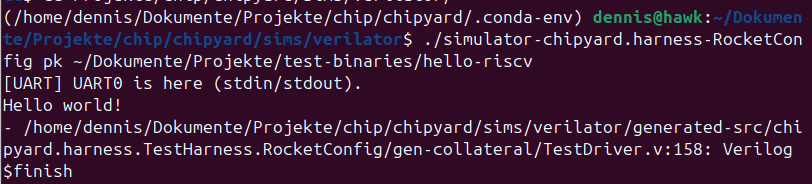
\includegraphics[scale=0.4]{testSuccess.png}
\end{figure}
\\\\
There are already different examples of code within chipyard, that can be run by verilator. More about this can be found under (2.1.5):\\
\url{https://chipyard.readthedocs.io/en/stable/Simulation/Software-RTL-Simulation.html}\\
It is possible to run the example code with the last command mentioned above. There is actually no use of "pk", you can leave this out in this case.\\\\
NOTE: It could be neccesary to execute \textit{cmake .} after executing \textit{make} in the "tests" directory of chipyard. After this you can go on with the instructions in the documentation.

\subsection*{Functional Simulation}
This simulation can be accomplished with \textbf{Spike} (or with Qemu). In this case only the 
RISCV instruction-architecture is simulated. This means that the instructions will be executed 
following the RISCV specification. It shows if the simulated program works correctly in terms 
of logic and architecture.\\
The command to use spike is:\\
\textit{spike pk "the-whole-path-to-your-.elf-file-starting-at-home-directory"}\\\\
You don't need to add the whole path if you are in the directory which contains the file you want to execute. In this case you just need to add the file.
If you want to execute the example code in tests from the chipyard directory with spike, leave out the "pk".


\section*{Algorithms in Simulation}
\subsection*{Fast Fourier Transformation}
The Fast Fourier Transformation was implemented with the help of FFTW (\url{https://www.fftw.org/}). In my case, it was neccesary to install it manually with the following commands:\\
\begin{verbatim}
    wget http://www.fftw.org/fftw-3.3.10.tar.gz

    tar xzf fftw-3.3.10.tar.gz

    cd fftw-3.3.10

    export CC=riscv64-unknown-elf-gcc

    export AR=riscv64-unknown-elf-ar

    export RANLIB=riscv64-unknown-elf-ranlib

    export HOST=riscv64-unknown-elf

    ./configure --host=$HOST --enable-static --disable-shared --prefix=$(pwd)/install

    make -j4

    make install
\end{verbatim}
To follow the instructions you need the following files:  image.py, fft\_output.txt, image\_data.h, fftw.c, gen\_freq\_pic.c and an image (e.g. test.png). All of these files should be in the
same directory.\\
The first step is to use the Python script to transform a picture into an array of values with 
the following command. You will be asked for a name of an image. You have to enter the whole name of the image including the ending (e.g. ".png").\\
\begin{verbatim}
    python3 image.py
\end{verbatim} 
The data created by the python script is added in the "image\_data.h" file. Everytime you choose a new image, the data in this file will be overwritten.\\
After you generated the data for the image, you can compile the FFT code with the following command:\\
\begin{verbatim}
    riscv64-unknown-elf-gcc -static 
    -I./fftw-3.3.10/install/include 
    -L./fftw-3.3.10/install/lib 
    -o fftw.elf fftw.c -lfftw3 -lm
\end{verbatim}
This will generate the executeable file for the simulation. Note that the conda environment needs to be activated and execute "source env.sh" in the chipyard directory. In the next step you can simulate this with spike:\\
\begin{verbatim}
    spike pk fftw.elf
\end{verbatim}
The output of the execution is written to the file "fft\_output.txt", which contains a huge amount of lines.\\
The code in "gen\_freq\_pic.c" serves the visualiztion of the simulation output. Therefore first compile this code with (only neccesary once):\\
\begin{verbatim}
    gen_freq_pic.c -o gen_freq_pic -lfftw3 -lm
\end{verbatim}
And then execute with:\\
\begin{verbatim}
    ./gen_freq_pic
\end{verbatim}
\subsection*{Edge Detection}
To perform edge detection in simulation you need the following files in the same directory: image.py, edge.c, image\_data.h, stb\_image.h, stb\_image\_write.h and an image (like test.png).\\
The files stb\_image.h and stb\_image\_write.h are added via:\\
\begin{verbatim}
    wget https://raw.githubusercontent.com/nothings/stb/master/stb_image.h
    wget https://raw.githubusercontent.com/nothings/stb/master/stb_image_write.h
\end{verbatim}
The first step is to use the Python script to transform a picture into an array of values with 
the following command. You will be asked for a name of an image. You have to enter the whole name of the image including the ending, in this case the endig needs always to be ".jpg" for the simulation.\\
\begin{verbatim}
    python3 image.py
\end{verbatim} 
The data created by the python script is added in the "image\_data.h" file. Everytime you choose a new image, the data in this file will be overwritten.\\
After you generated the data for the image, you can compile the FFT code with the following command:\\
\begin{verbatim}
    riscv64-unknown-elf-gcc -static  -o edge.elf edge.c  -lm
\end{verbatim}
This will generate the executeable file for the simulation. Note that the conda environment needs to be activated and execute "source env.sh" in the chipyard directory. In the next step you can simulate this with spike:\\
\begin{verbatim}
    spike pk edge.elf
\end{verbatim}
The simulation will automatically generate a new image which shows the the result of the edge detection. The image for the result is saved in "edges.png".
\subsection*{Optical Flow}
- measuring the movement of object in a scene, approximation of movement between to frames\\
- assumptions are neccesary: \\
1. brightness of an image point remains constant over time\\
2. displacemant and time step are very small\\
- maybe use of OpenCV \\
- Lucas Kanade Method: Assumption: for each pixel assume Motionfield (hence Optical Flow) is constant within a small neighborhood



\section*{Further Notes}
Use Rocket Chip on FPGA:\\
- Rocket Chip can be configured but as defualt it has AXI connections (and a debug connection)\\
- it is possible to define a differnt configuration and with this you can change periphery\\
- it is neccessary to convert the connections (e.g. AXI to PCIe) when using a FPGA\\
- firesim has predefined configurations for specfic FPGAs\\
source: \url{https://github.com/chipsalliance/rocket-chip/issues/1594}
- use of "Vivado" (Installation neccessary)\\
- within chipyard it is possible to build a bitstream\\
-> chisel is converted to verilog, this runs through vivado to create a bitstream 
}
\end{document}